\documentclass[12pt]{article}
\usepackage[margin=1in]{geometry}
\usepackage{graphicx}
\usepackage{amsmath}
\usepackage{tikz}
\usepackage{hyperref}
\usepackage{enumitem}

\newcommand{\fromlectures}{{\\ \color{blue} \hspace*{\fill}(from lecture slides)} \\}
\newcommand{\bydefn}{{\\ \color{blue} \hspace*{\fill}(by definition)} \\}
\newcommand{\given}{{\\ \color{blue} \hspace*{\fill}(given)} \\}
\newcommand{\rtp}{{\\ \color{blue} \hspace*{\fill}(required to prove)} \\}

\newcommand{\f}[1]{o_{#1}x_{#1}y_{#1}z_{#1}}
\newcommand{\rx}[1]{\begin{bmatrix} 1 & 0 & 0 & 0 \\ 0 & cos(#1) & -sin(#1) & 0 \\ 0 & sin(#1) & cos(#1) & 0 \\ 0 & 0 & 0 & 1 \end{bmatrix}}
\newcommand{\rz}[1]{\begin{bmatrix} cos(#1) & -sin(#1) & 0 & 0 \\ sin(#1) & cos(#1) & 0 & 0 \\ 0 & 0 & 1 & 0 \\ 0 & 0 & 0 & 1 \end{bmatrix}}
\newcommand{\iden}{\begin{bmatrix} 1 & 0 & 0 & 0 \\ 0 & 1 & 0 & 0 \\ 0 & 0 & 1 & 0 \\ 0 & 0 & 0 & 1 \end{bmatrix}}
\newcommand{\trans}[3]{\begin{bmatrix} 1 & 0 & 0 & #1 \\ 0 & 1 & 0 & #2 \\ 0 & 0 & 1 & #3 \\ 0 & 0 & 0 & 1 \end{bmatrix}}

\title{CSci 5551 - HW3}
\author{Yashasvi Sriram Patkuri\\patku001@umn.edu}

\begin{document}
\maketitle
\pagebreak

\section{}
The robot arm has 3 DOF as illustrated in the Figure \ref{fig:q1.1}.
I am assuming that length of link 3 is $L_3$ since it is not mentioned in the figure.
\given

\begin{figure}[h]
  \centering
  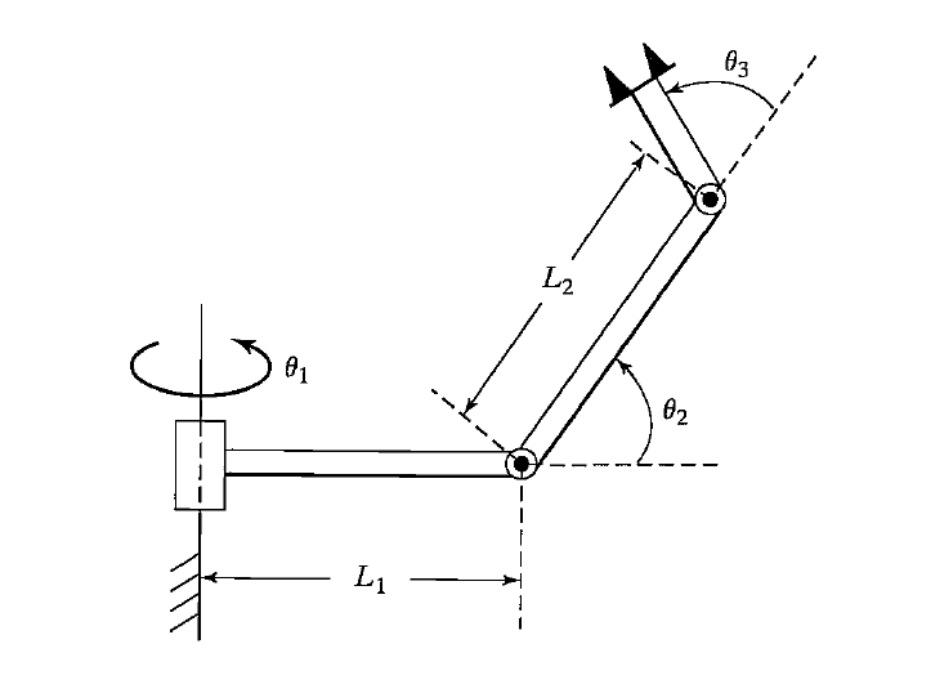
\includegraphics[width=0.6\textwidth]{q1.png}
  \caption{3DOF robot arm}
  \label{fig:q1.1}
\end{figure}

Assigning frames according to DH convention we have,
\fromlectures
\begin{figure}[h]
  \centering
  \begin{tikzpicture}[x=1cm, y=1cm, z=-0.6cm]
    % F1
    \draw [->]       (0, 0) -- (2, 0) node [right] {$x_1$};
    \draw [->]       (0, 0) -- (0, 2) node [left] {$z_1$};
    % F2
    \draw [->]       (4, 0) -- (6, 0) node [right] {$x_2$};
    \draw            (4, 0) circle (0.15cm);
    \draw [fill]     (4, 0) circle (0.07cm) node [left] {$z_2$};
    % F3
    \draw [->]       (6, 2) -- (7.414, 3.414) node [right] {$x_3$};
    \draw            (6, 2) circle (0.15cm);
    \draw [fill]     (6, 2) circle (0.07cm) node [left] {$z_3$};
    % F4
    \draw [->]       (5, 4) -- (3.656, 5.514) node [right] {$x_4$};
    \draw            (5, 4) circle (0.15cm);
    \draw [fill]     (5, 4) circle (0.07cm) node [right] {$z_4$};
  \end{tikzpicture}
  \caption{DH frame assignment}
  \label{fig:q1.2}
\end{figure}
\begin{enumerate}[nolistsep]
  \item The z-axes are along the axes of rotation.
  \item The choice of $z_4$ is free, so it is chosen to be parallel to $z_3$ for simplicity.
  \item The choice of $x_1$ is free, so it chosen in the direction of $x_2$ for simplicity.
  \item $x_2$ lies along the common normal to $z_1$ and $z_2$ which is unique.
  \item There are many common normal to $z_2$ and $z_3$ as they are parallel, so $x_3$ is chosen to be in the plane of paper for simplicity.
  \item $x_4$ is chosen in a similar manner.
  \item Each y-axis (not shown) just form a right handed coordinate system with respective frame.
\end{enumerate}

\subsubsection*{DH parameters}
The DH parameters for the frames shown in Figure \ref{fig:q1.2} are as follows
\begin{center}
\begin{tabular}{ c | c c c c }
 \hline
 $F_i \to F_j$ & $\theta$ & d & r & $\alpha$ \\
 \hline
 $1 \to 2$ & $\theta_1$ & 0 & $L_1$ & $90^{\circ}$ \\
 $2 \to 3$ & $\theta_2$ & 0 & $L_2$ & $0^{\circ}$ \\
 $3 \to 4$ & $\theta_3$ & 0 & $L_3$ & $0^{\circ}$ \\
 \hline
\end{tabular}
\end{center}

\subsubsection*{Transformation from $F_1$ to $F_3$}
\[
  T_{13} \equiv T_{12} * T_{23}
\]
$T_{12}, T_{23}$ can be constructed using DH parameters.
Given frame i and frame j with DH parameters [ $\theta$, d, r, $\alpha$ ] the transformation matrix is
\[
  T_{i,j} \equiv Rot_{z,\theta} * Trans_{z, d} * Trans_{x, r} * Rot_{x, \alpha}
\]
\fromlectures
Consider $T_{12}$
\[
  T_{12} \equiv Rot_{z,\theta_1} * Trans_{z, 0} * Trans_{x, L_1} * Rot_{x, 90^{\circ}}
\]
\[
  T_{12} \equiv \rz{\theta_1} * \trans{0}{0}{0} * \trans{L_1}{0}{0} * \rx{90^{\circ}}
\]
\[
  T_{12} \equiv \rz{\theta_1} * \trans{L_1}{0}{0}
    * \begin{bmatrix} 1 & 0 & 0 & 0 \\ 0 & 0 & -1 & 0 \\ 0 & 1 & 0 & 0 \\ 0 & 0 & 0 & 1 \end{bmatrix}
\]
\[
  T_{12} \equiv \rz{\theta_1}
  * \begin{bmatrix} 1 & 0 & 0 & L_1 \\ 0 & 0 & -1 & 0 \\ 0 & 1 & 0 & 0 \\ 0 & 0 & 0 & 1 \end{bmatrix}
\]
\[
  T_{12} \equiv
  \begin{bmatrix} c\theta_1 & 0 & s\theta_1 & L_1c\theta_1 \\ s\theta_1 & 0 & -c\theta_1 & L_1s\theta_1 \\ 0 & 1 & 0 & 0 \\ 0 & 0 & 0 & 1 \end{bmatrix}
\]

Consider $T_{23}$
\[
  T_{23} \equiv Rot_{z,\theta_2} * Trans_{z, 0} * Trans_{x, L_2} * Rot_{x, 0^{\circ}}
\]
\[
  T_{23} \equiv \rz{\theta_2} * \trans{0}{0}{0} * \trans{L_2}{0}{0} * \rx{0^{\circ}}
\]
\[
  T_{23} \equiv \rz{\theta_2} * \trans{0}{0}{0} * \trans{L_2}{0}{0} * \iden
\]
\[
  T_{23} \equiv \rz{\theta_2} * \trans{L_2}{0}{0}
\]
\[
  T_{23} \equiv
  \begin{bmatrix} c\theta_2 & -s\theta_2 & 0 & L_2c\theta_2 \\ s\theta_2 & c\theta_2 & 0 & L_2s\theta_2 \\ 0 & 0 & 1 & 0 \\ 0 & 0 & 0 & 1 \end{bmatrix}
\]

\[
  T_{13} \equiv T_{12} * T_{23}
\]
Substituting $T_{12}, T_{23}$ we have,
\[
  T_{13} \equiv
  \begin{bmatrix} c\theta_1 & 0 & s\theta_1 & L_1c\theta_1 \\ s\theta_1 & 0 & -c\theta_1 & L_1s\theta_1 \\ 0 & 1 & 0 & 0 \\ 0 & 0 & 0 & 1 \end{bmatrix}
  *
  \begin{bmatrix} c\theta_2 & -s\theta_2 & 0 & L_2c\theta_2 \\ s\theta_2 & c\theta_2 & 0 & L_2s\theta_2 \\ 0 & 0 & 1 & 0 \\ 0 & 0 & 0 & 1 \end{bmatrix}
\]
\[
  T_{13} \equiv
  \begin{bmatrix}
    c\theta_1c\theta_2 & -c\theta_1s\theta_2 & s\theta_1 & L_2c\theta_1c\theta_2 + L_1c\theta_1 \\
    s\theta_1c\theta_2 & -s\theta_1s\theta_2 & -c\theta_1 & L_2s\theta_1c\theta_2 + L_1s\theta_1 \\
    s\theta_2 & c\theta_2 & 0 & L_2s\theta_2 \\
    0 & 0 & 0 & 1
  \end{bmatrix}
\]

\pagebreak

\section{}
\section{}
\section{}

\end{document}
